\documentclass[10pt]{article}
\usepackage[utf8]{inputenc}
\usepackage[english]{babel}
\usepackage[font=small,labelfont=bf]{caption}
\usepackage{geometry}
\usepackage{natbib}
\usepackage{pxfonts}
\usepackage{graphicx}
\usepackage{newfloat}
\usepackage{setspace}
%\doublespacing

\newcommand{\argmax}{\mathop{\mathrm{argmax}}\limits}

\title{\textit{Supplemental figures for}: A Gaussian process model of human electrocorticographic data} 
\author{
  Lucy L. W. Owen$^{1}$,
  Andrew C. Heusser$^{1, 2}$, and
  Jeremy R. Manning$^{1\ast}$\\\\
$^{1}$Department of Psychological and Brain Sciences, Dartmouth College,\\
Hanover, NH 03755, USA\\
$^{2}$Akili Interactive,\\
Boston, MA 02110, USA}

\bibliographystyle{apa}

\begin{document}
\maketitle

\setcounter{equation}{0}
\setcounter{figure}{0}
\setcounter{table}{0}
\setcounter{page}{1}
\setcounter{section}{0}
\makeatletter
\renewcommand{\theequation}{S\arabic{equation}}
\renewcommand{\thefigure}{S\arabic{figure}}
\renewcommand{\bibnumfmt}[1]{[S#1]}
\renewcommand{\citenumfont}[1]{S#1}


\begin{figure}[b!]
\centering
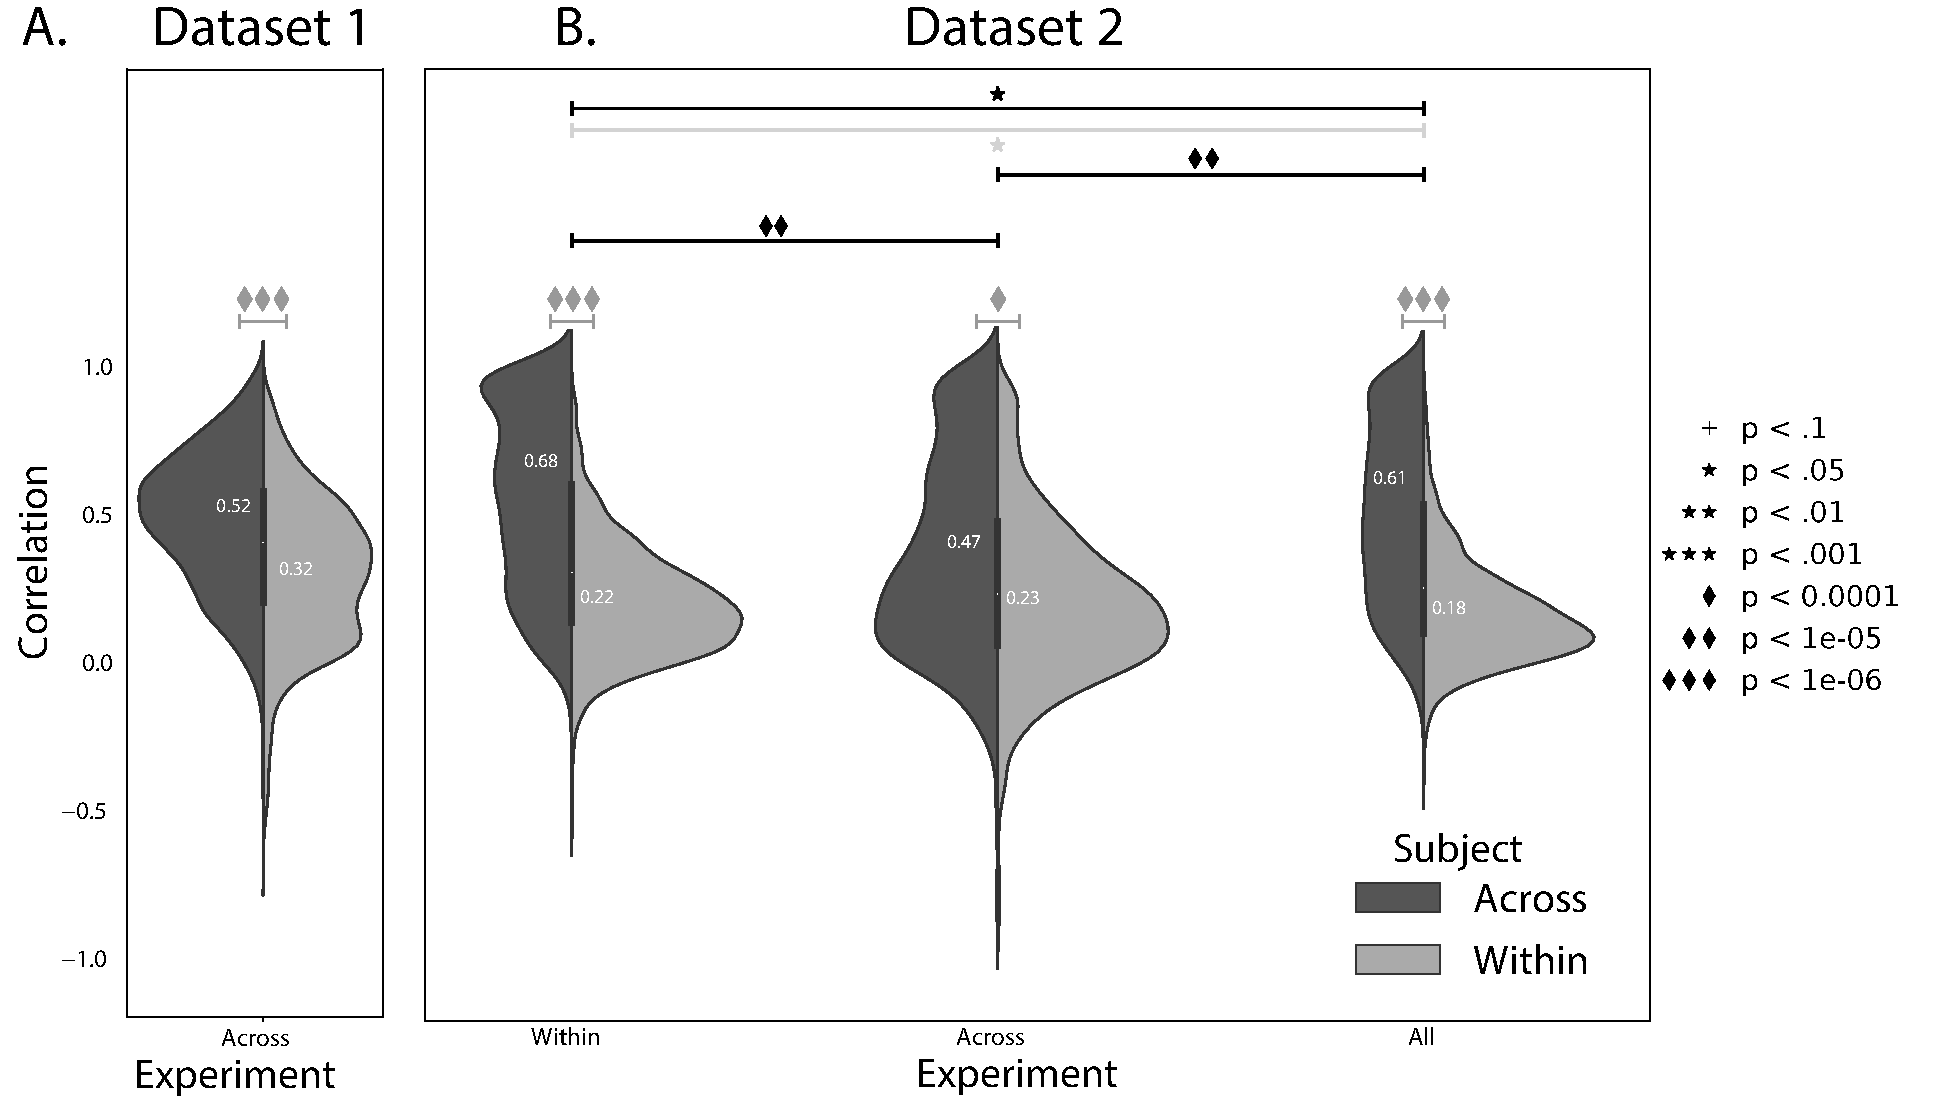
\includegraphics[width=0.6\textwidth]{figs/supplemental_1}
\caption{\textbf{Reconstruction quality for Datasets 1 and 2.}
  \textbf{A. Distributions of correlations between observed versus
    reconstructed activity by electrode, for Dataset 1.} The split
  violin plot reflects the same data as Figure~3A, presented here for
  comparison.  \textbf{B. Distributions of correlation between
    observed versus reconstructed activity by electrode, for Dataset
    2.}  The right-most split violin plot (``All'') reflects the same
  data as Figure~3B, presented here for comparison.  The ``Within''
  plot reflects the same analyses, but limited to models that were
  trained and tested on only one of the Dataset 2 experiments at a
  time.  The ``Across'' plot reflects the same analyses, but limited
  to models that were trained and tested on \textit{different} Dataset
  2 experiments.  All plots: the dark gray distributions denote
  across-subject correlations (model trained on all but one patient
  and tested on the held-out patient), and the medium gray
  distributions denote within-subject correlations (model trained on
  all but one electrode from one patient, and tested on the held-out
  electrode).  The horizontal bars denote $t$-tests between the
  corresponding distributions (after $z$-transforming the
  correlations), and the white numbers reflect the distribution means.
  The symbols denote the corresponding $p$-values of those statistical
  tests.}
\label{fig:supplemental_1}
\end{figure}


\begin{figure}[p]
\centering
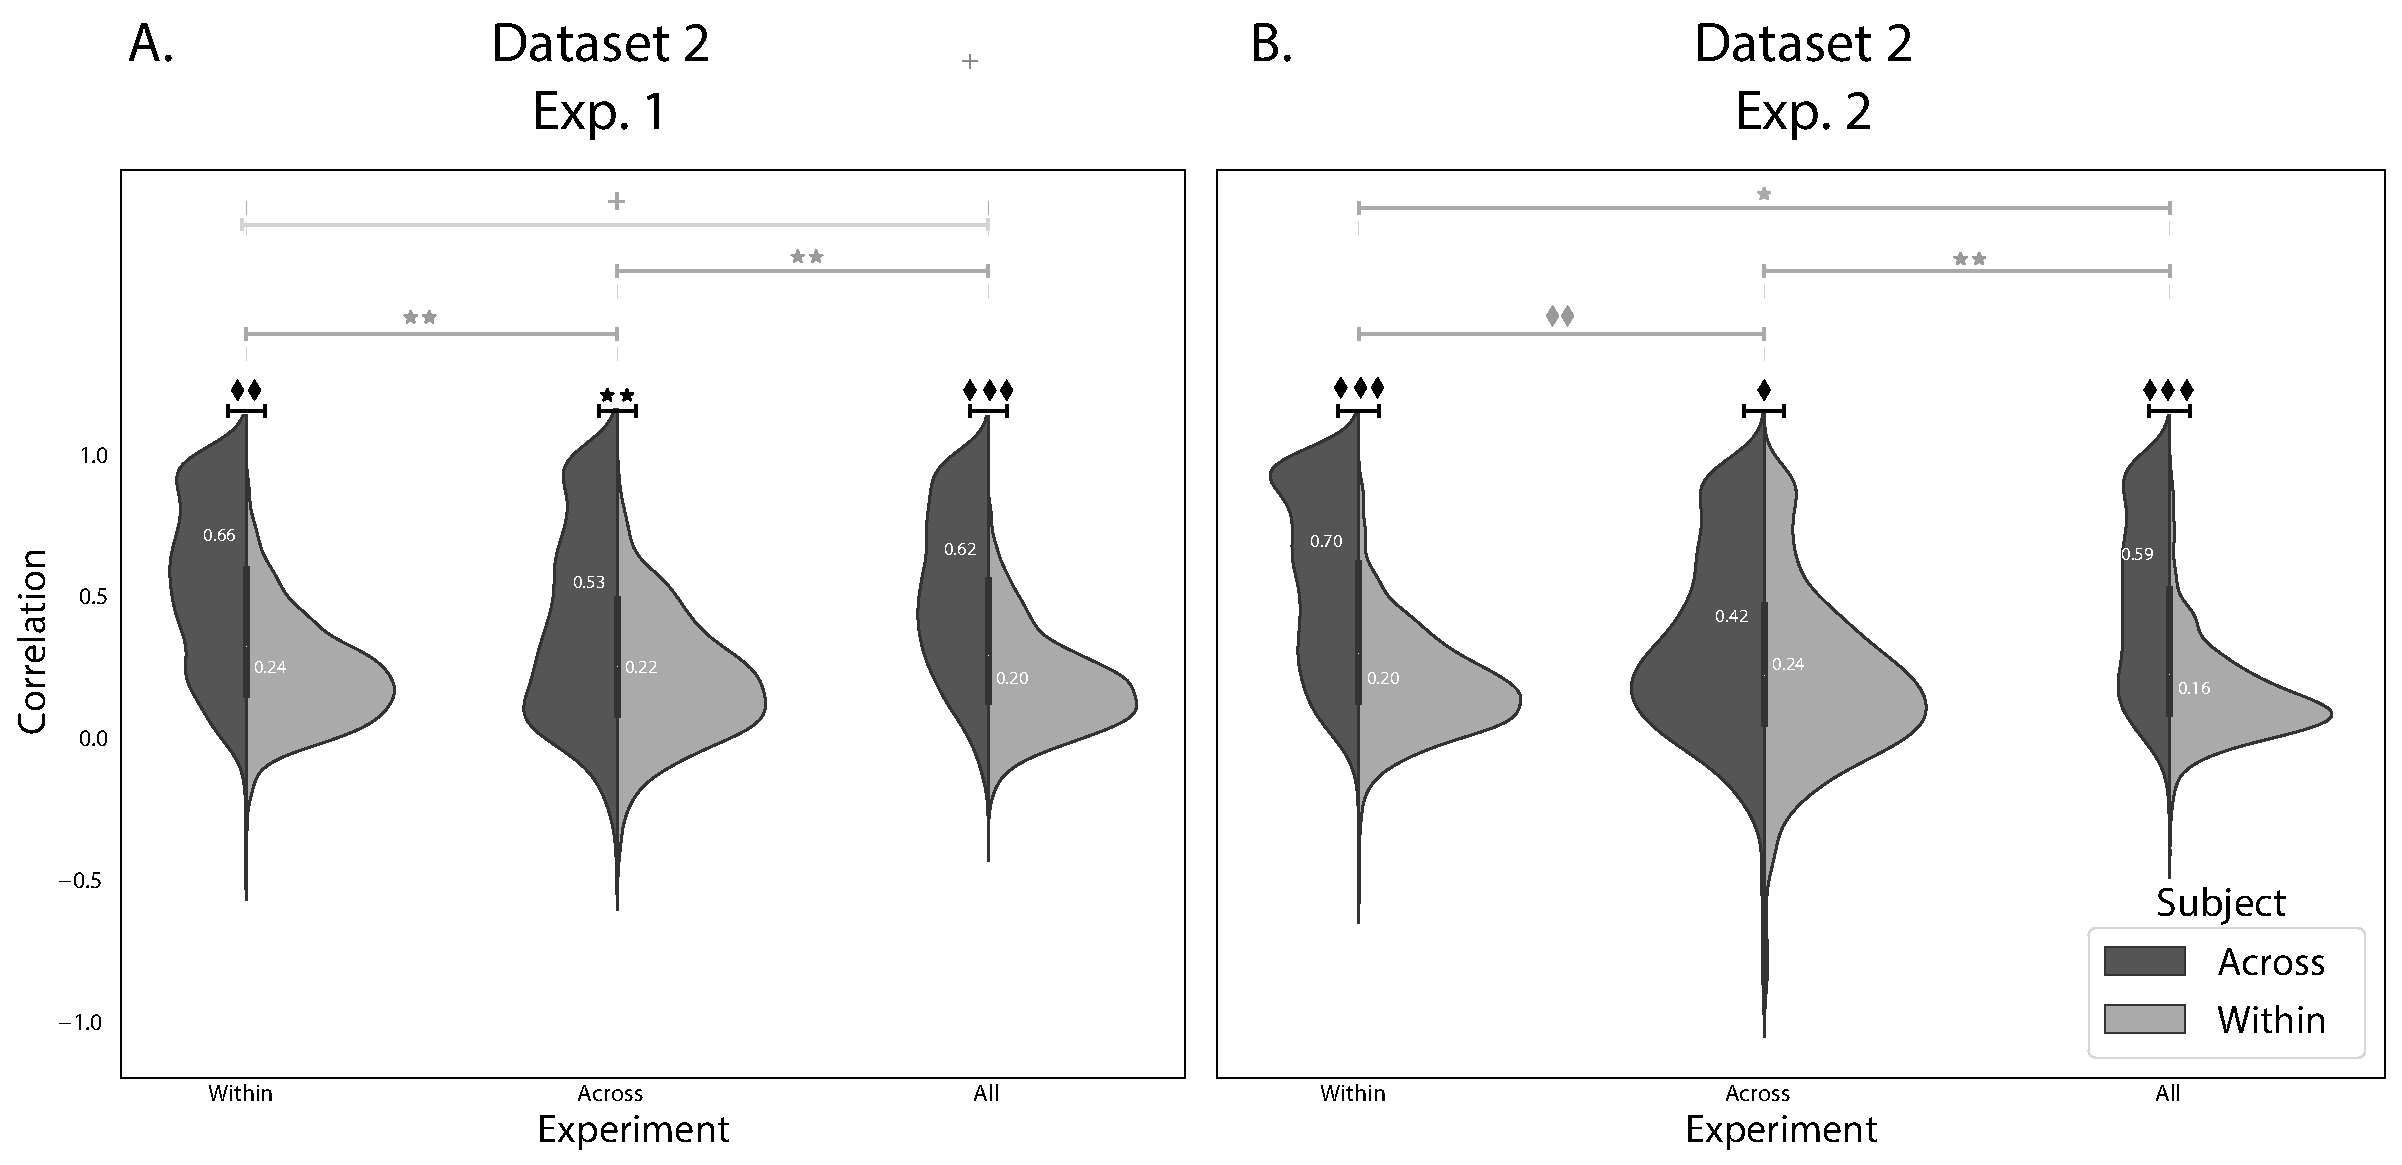
\includegraphics[width=\textwidth]{figs/supplemental_2}
\caption{\textbf{Reconstruction quality for Dataset 2,
    Experiments 1 and 2.} \textbf{A. Distributions of correlations
    between observed versus reconstructed activity by electrode, for
    Experiment 1.}  Each split violin plot and horizontal bar is in
  the same format as the plots in Figure~\ref{fig:supplemental_1}.
  ``Within'' denotes within-subject correlations (model trained on all
  but one electrode from one patient, and tested on the held-out
  electrode); ``Across'' denotes across-subject correlations (model
  trained an all but one patient and tested on the held-out patient);
  ``All'' denotes a model trained on all data from all patients,
  except for one held-out electrode (and tested on the held-out
  electrode).  \textbf{B. Distributions of correlations between
    observed versus reconstructed activity by electrode, for
    Experiment 2.}  All of the plots and bars are in the same format
  as those in Panel A.}
\label{fig:supplemental_2}
\end{figure}

\begin{figure}[p]
\centering
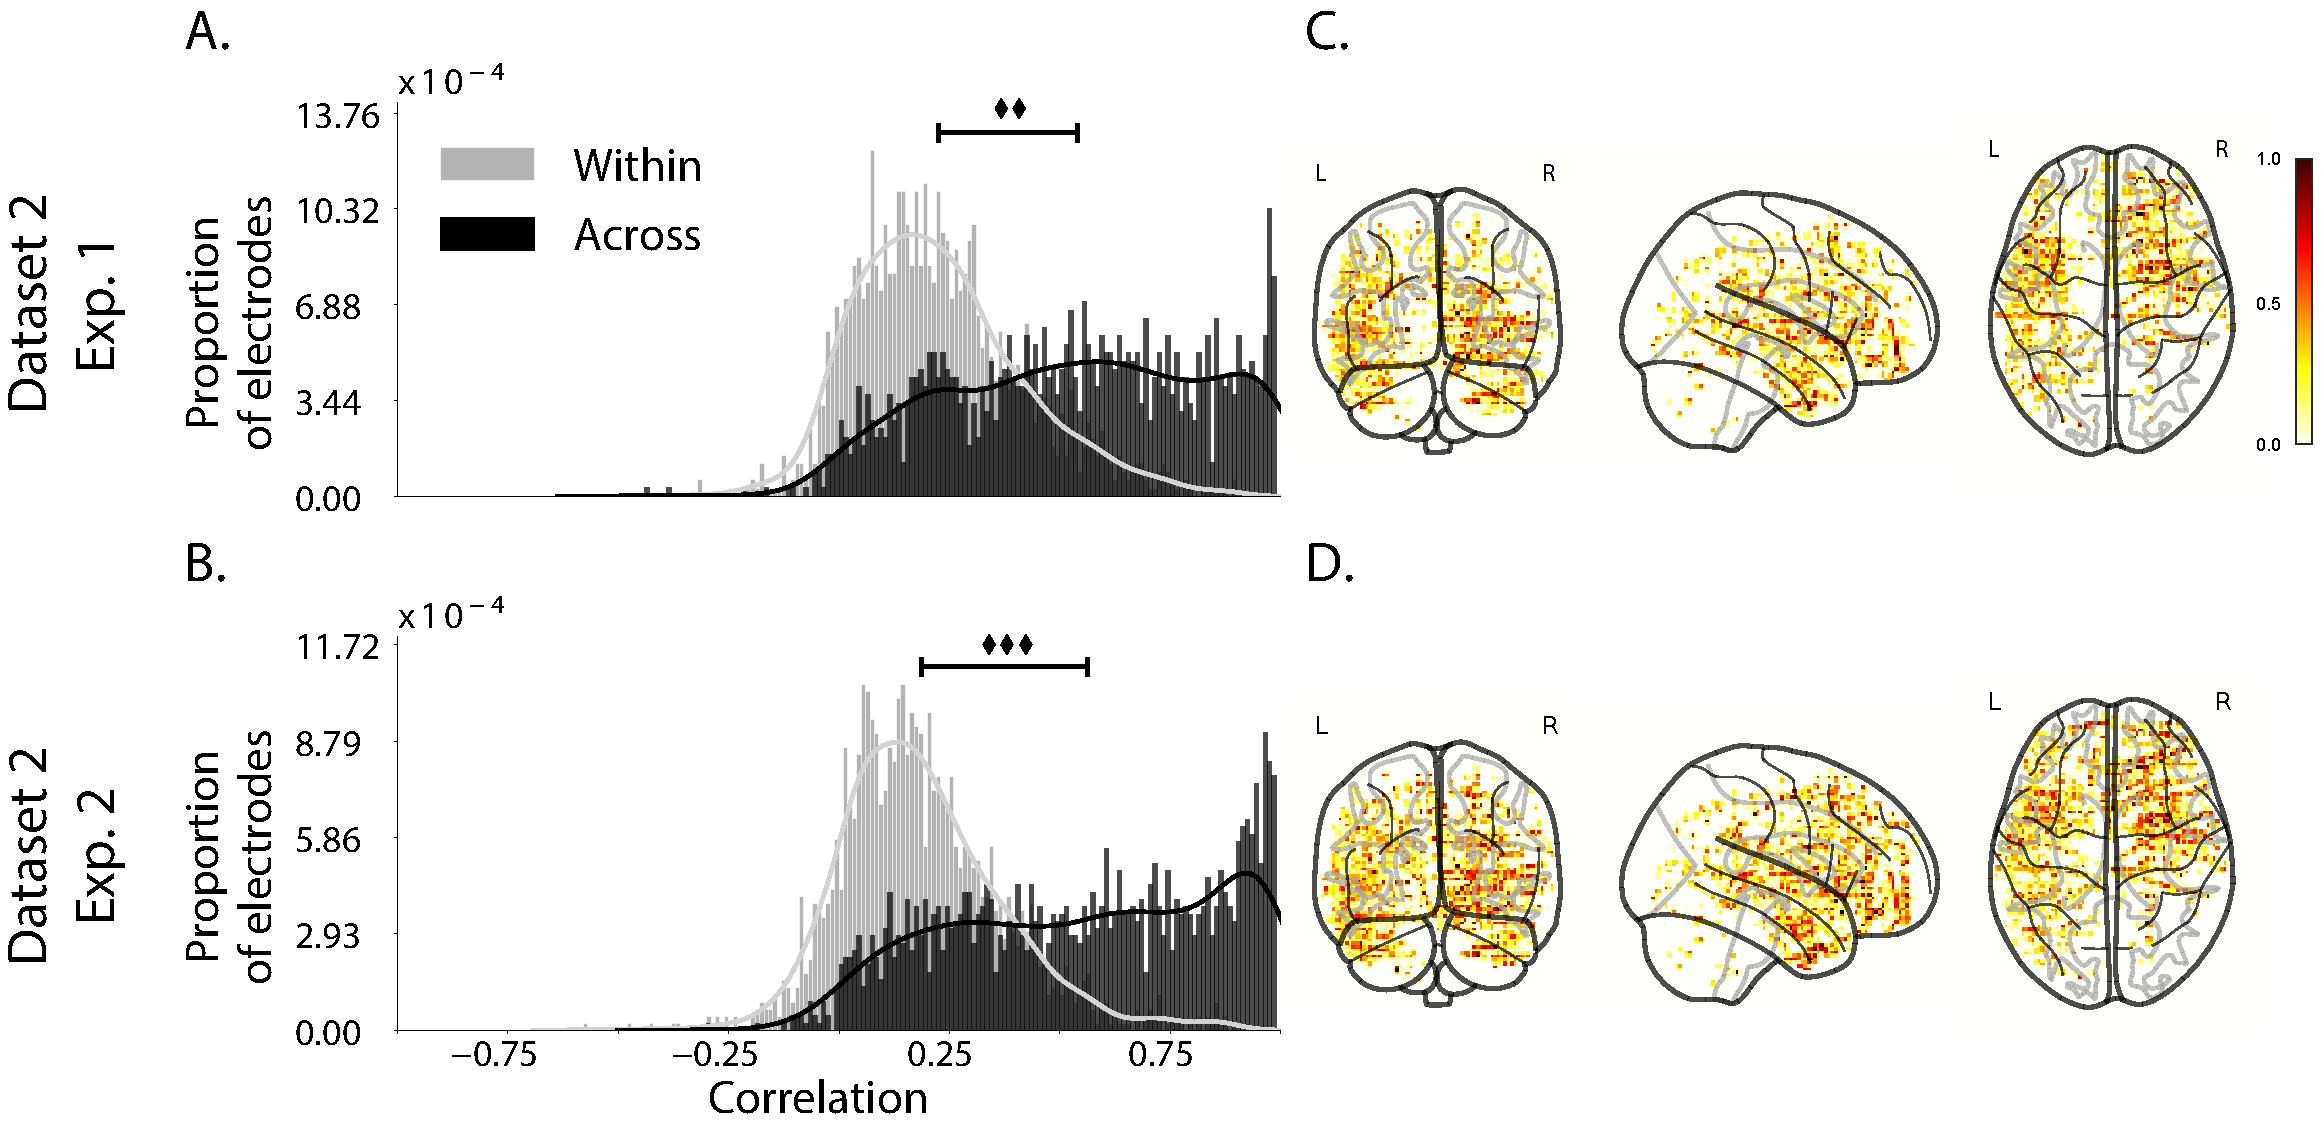
\includegraphics[width=\textwidth]{figs/supplemental_3}
\caption{\textbf{Reconstruction quality across all electrodes in two
      Dataset 2 experiments.}  \textbf{A. Distributions of correlations
      between observed versus reconstructed activity by electrode, for
      Experiment 1.}  Same format as Figure~3A and B, but reflects data shown
    in Figure~\ref{fig:supplemental_2}A (rightmost violin plot).
 \textbf{B. Distributions of correlations
      between observed versus reconstructed activity by electrode, for
      Experiment 2.}  Same format as Figure~3A and B, but reflects
    data shown in Figure~\ref{fig:supplemental_2}B (rightmost violin
    plot).  \textbf{C.--D.  Reconstruction
      performance by location.} Each dot reflects the location of a
    single implanted electrode from Dataset 2, Experiment 1 (Panel C)
    or Dataset 2, Experiment 2 (Panel D).  The dot colors denote the
    average within-experiment (across-session)
    correlation, using the across-patient correlation model, between
    the observed and reconstructed activity at the given electrode
    location.}
\label{fig:supplemental_3}
\end{figure}


\begin{figure}[p]
\centering
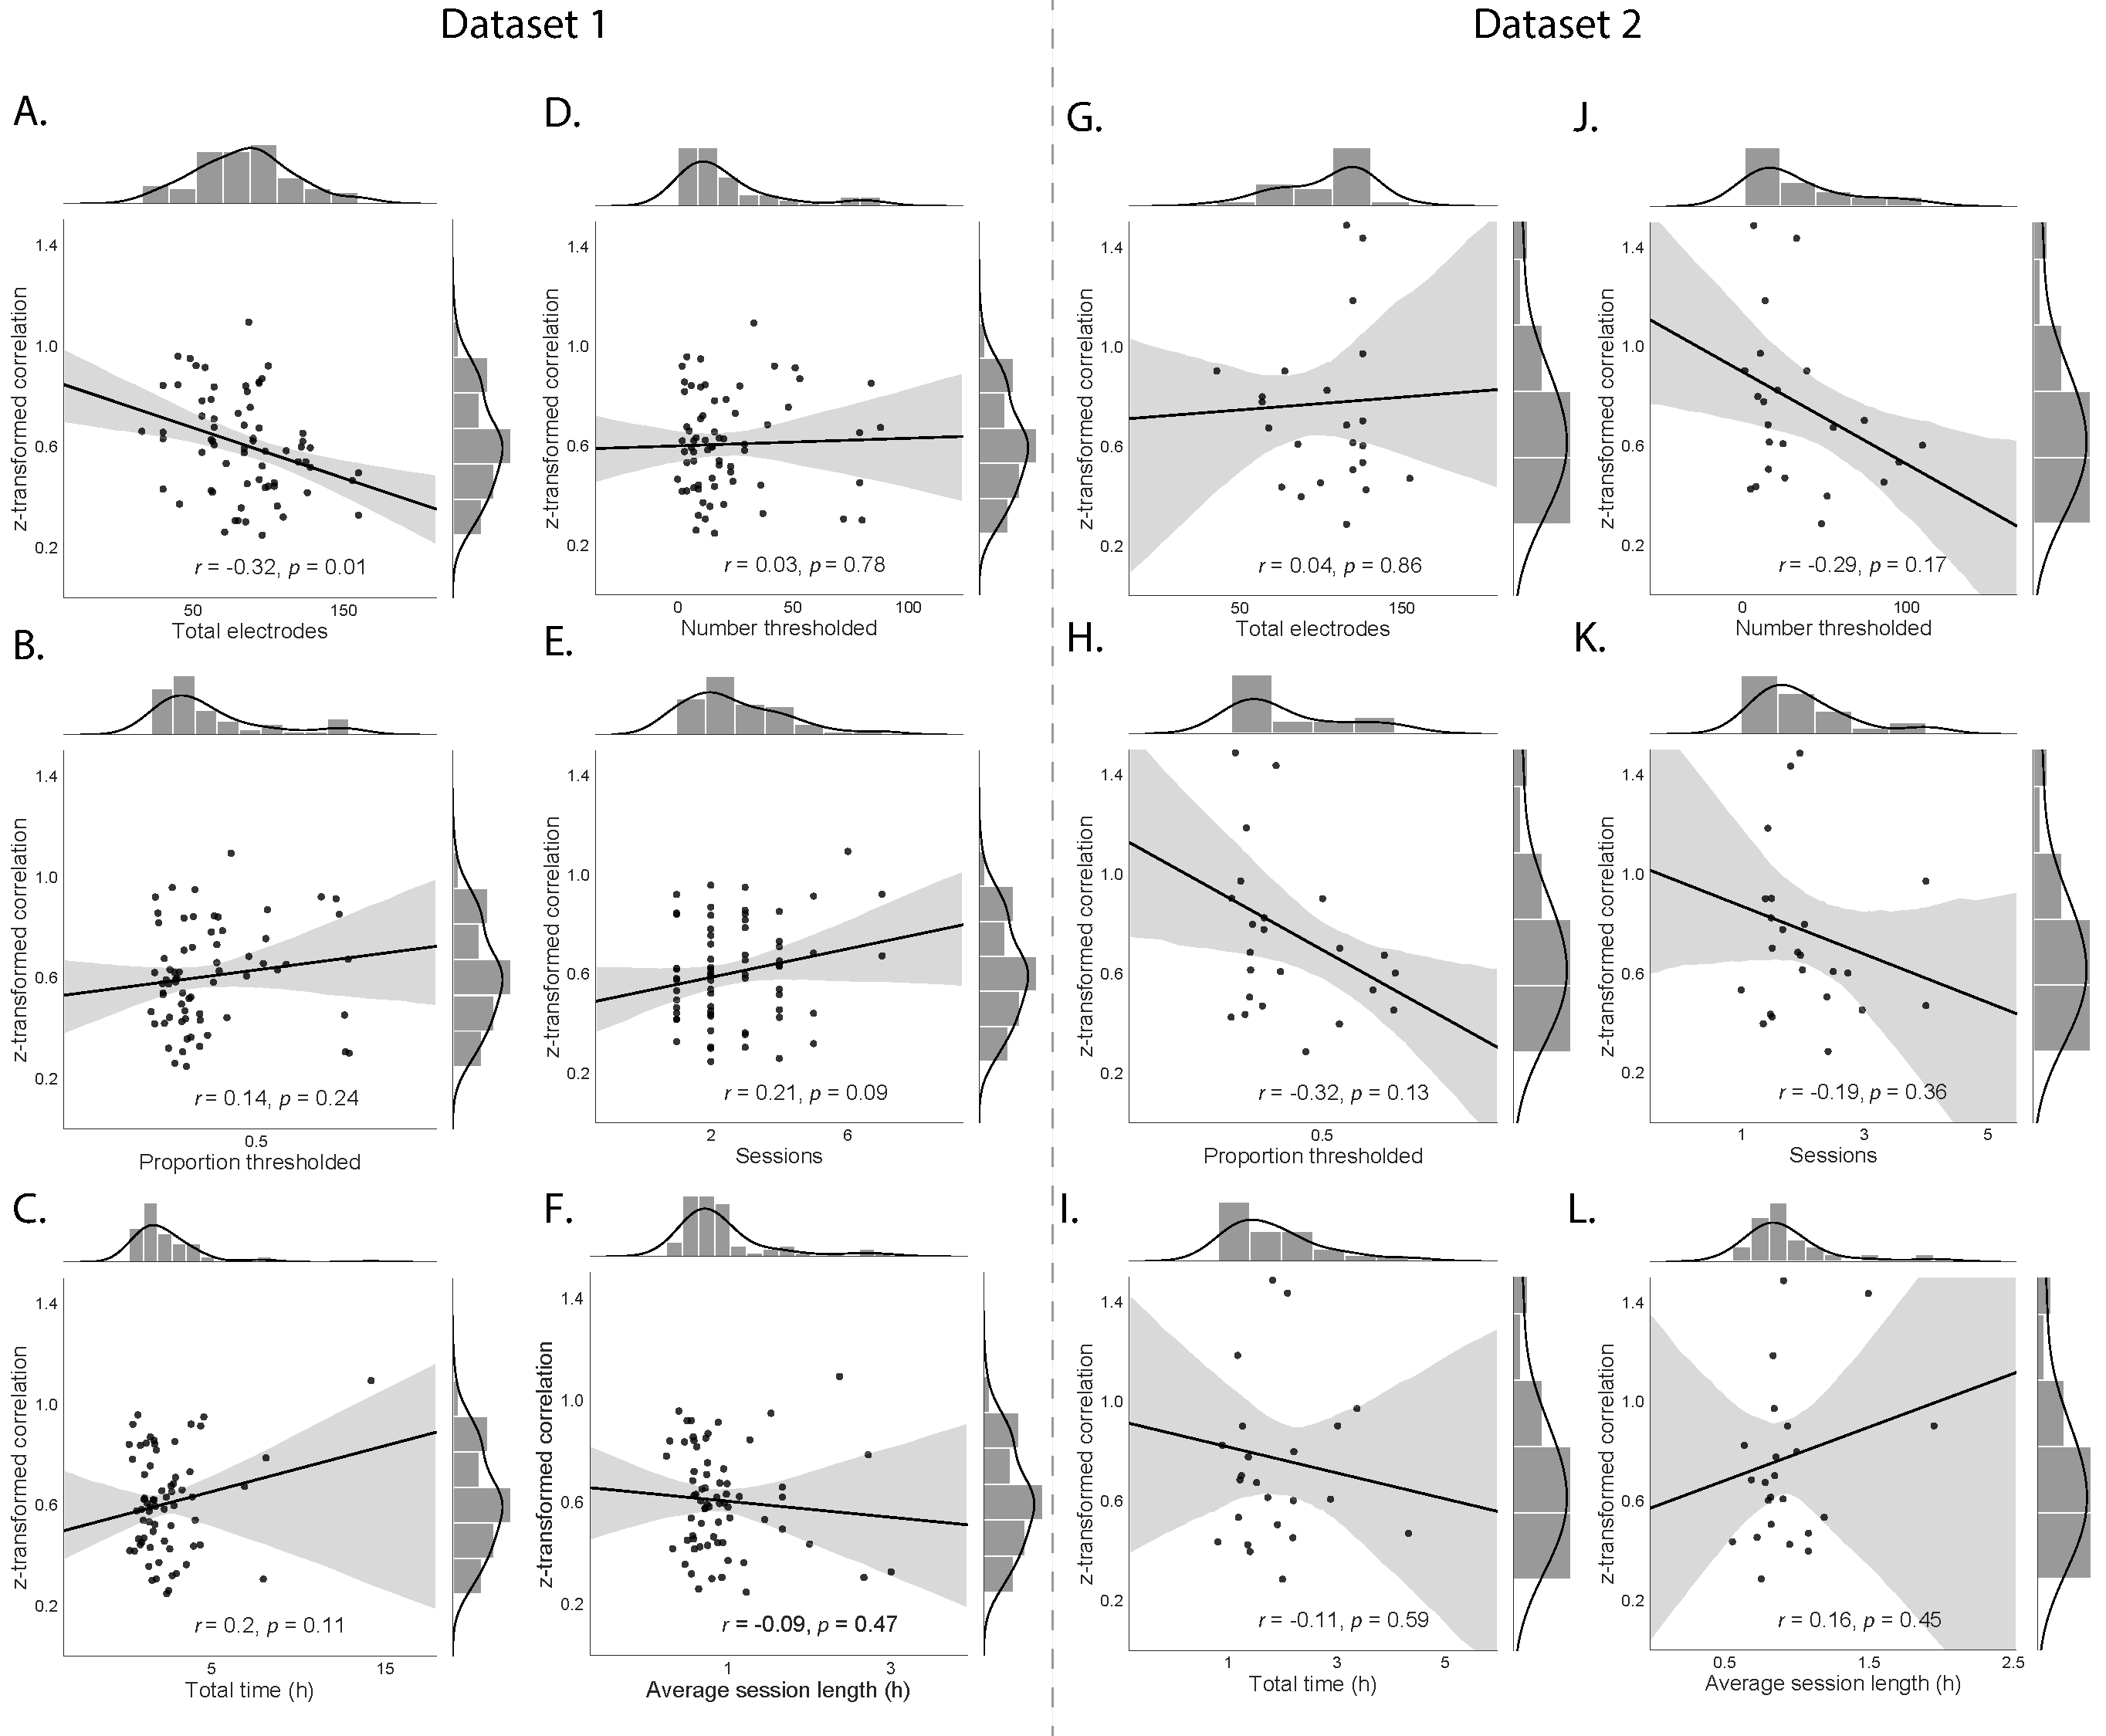
\includegraphics[width=\textwidth]{figs/supplemental_4}
\caption{\textbf{Reconstruction accuracy versus within-subject data
    features for two ECoG datasets.} \textbf{A.--F.  Features from
    Dataset 1.}  Features include: (\textbf{A.}) total number of
  electrodes implanted in each patient's brain, (\textbf{B.})
  per-patient number of electrodes that were filtered out due to
  having an maximum kurtosis greater than 10 across all recording
  sessions, (\textbf{C.})  per-patient proportion of electrodes that
  were filtered out due to having an average kurtosis greater than 10,
  (\textbf{D.})  per-patient number of recording sessions,
  (\textbf{E.}) per-patient total recording time (h), and
  (\textbf{F.}) per-patient average session length (h).
  \textbf{G.--L. Features from Dataset 2.}  Analogous format to Panels
  A--F.}
\label{fig:supplemental_4}
\end{figure}


\begin{figure}[ptb]
\centering
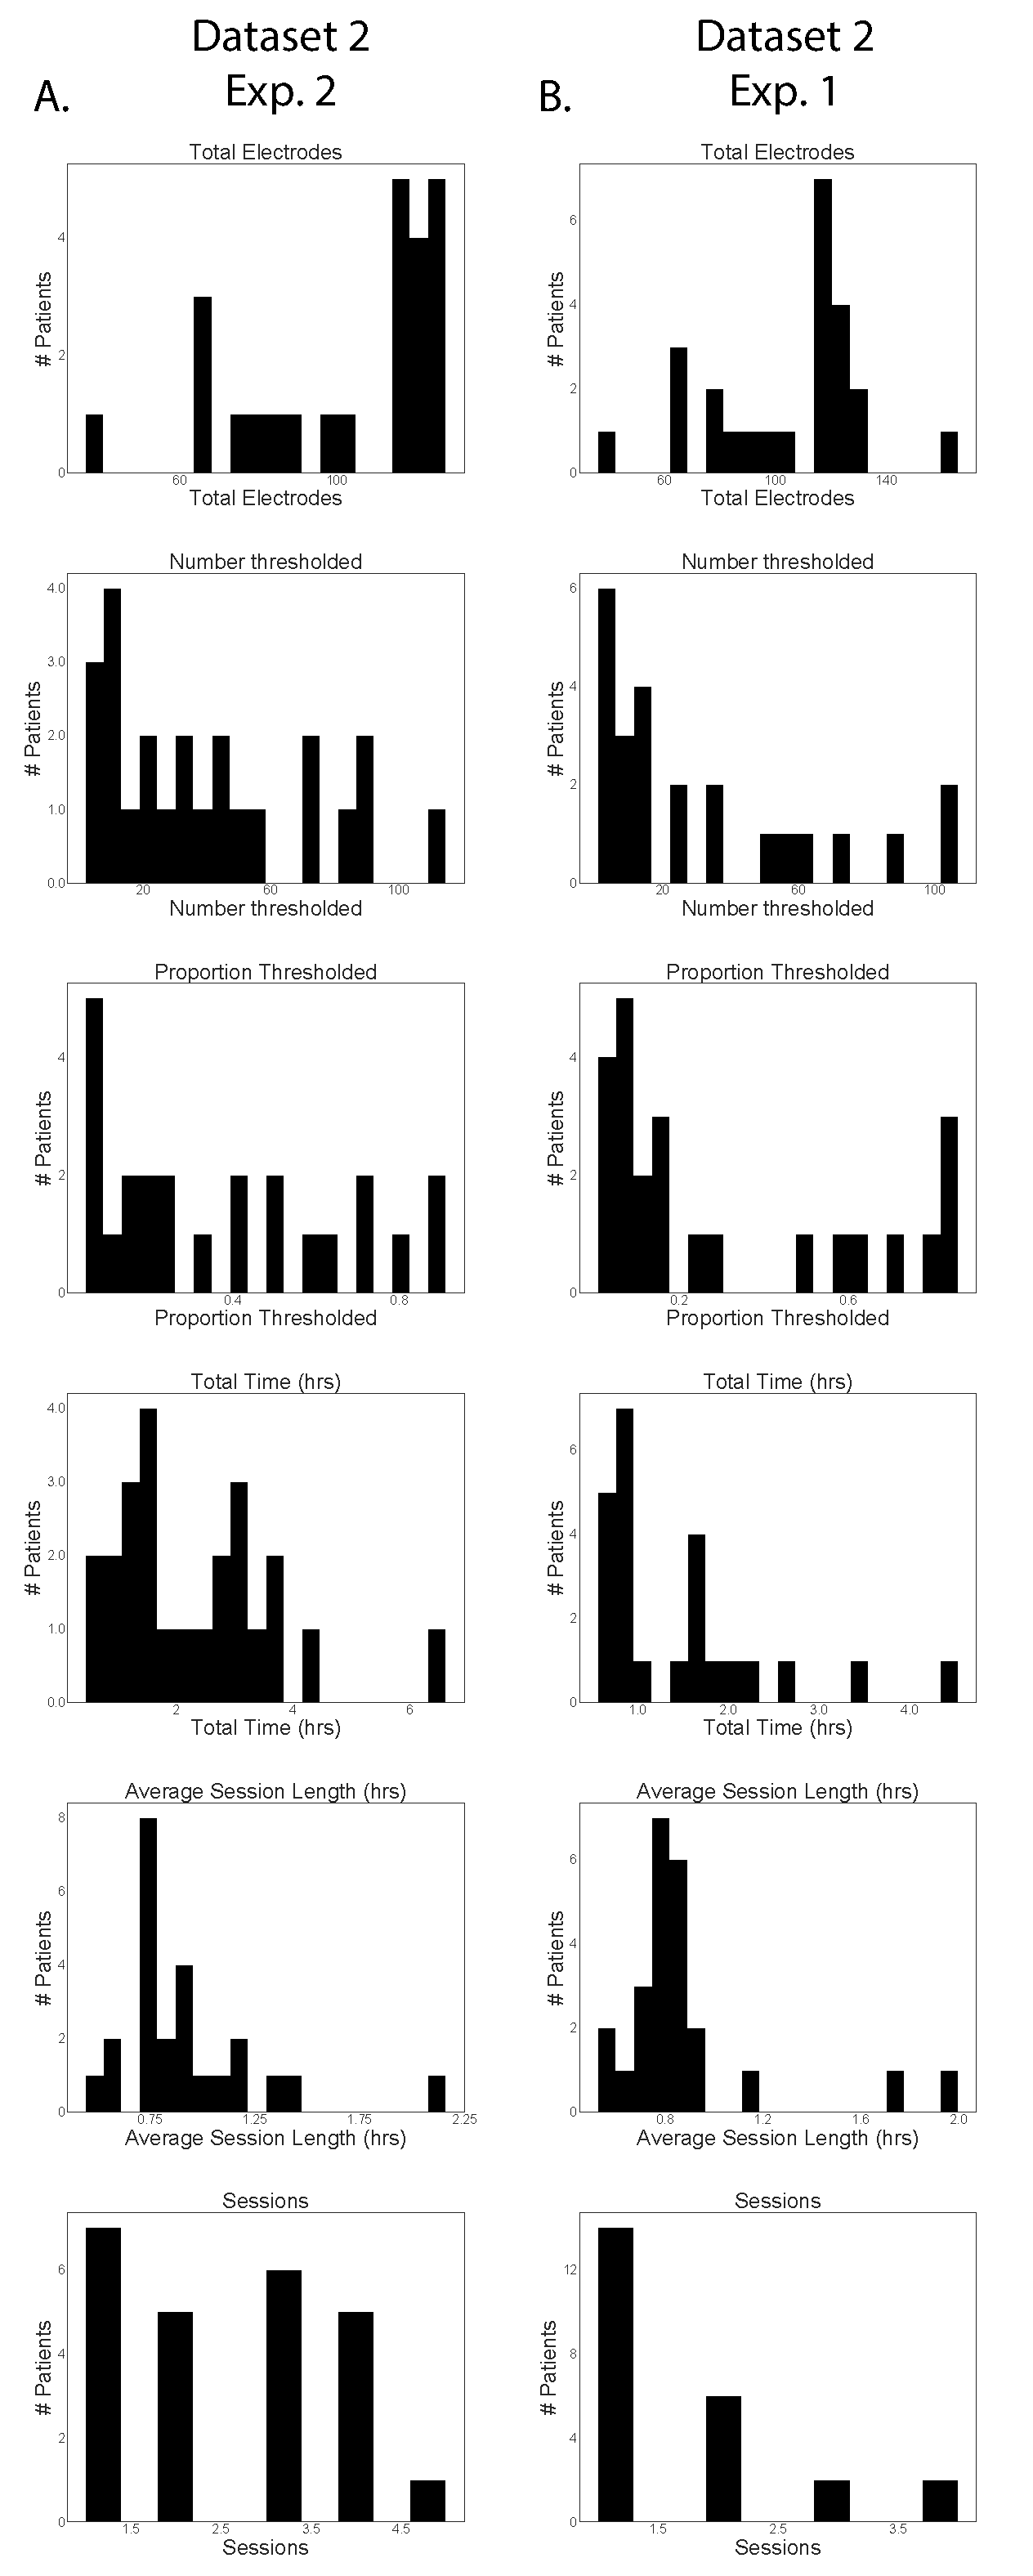
\includegraphics[width=\textwidth]{figs/supplemental_5}
\caption{\textbf{Most informative electrode locations.}  This map
  shows the region outlined in white from Figure~5 in greater detail.
  Across Datasets 1 and 2, electrodes in these locations were
  identified as yielding the (10\%) best reconstruction accuracies at
  \textit{other} locations throughout the brain.  The $x$-coordinates
  in each panel denote the positions of the sagittal slices in MNI space.}
\label{fig:supplemental_5}
\end{figure}


% \newpage
% \renewcommand{\refname}{Supplemental references}
% \bibliography{memlab}


\end{document}